
% tableau: gauche -> règle en anglais, droite -> rule en ASP

%%%%%%%%%%%%%%%%%%%%%%%%%%%%%%%%%%%%
\chapter{Learning rules for board Games}

In this chapter, we want to find some hypotheses that explain the rules of the two games described in the previous chapter.

\section{Different ways of learning the rules}

\subsection{Dependencies}

In the last chapter, we defined four predicates (\texttt{legal/3}, \texttt{can\_play/3}, \texttt{phase/2} and \texttt{finished/2}) in order to tell which actions are valid.

\smallskip

%TODO : cite paper bayesian networks
We will always keep the definition of \texttt{phase/2} given in the previous chapter, and we will learn the three others knowing the dependencies described in figure \ref{fig:general_dependencies} . All these \textit{dependency diagrams} follow the convention of Bayesian networks \citep{pearl2014probabilistic}: if there is an arrow going from a predicate \texttt{a} to a predicate \texttt{b}, then \texttt{b} depends on \texttt{a}. In other words, the predicate \texttt{a} appears in the definition of \texttt{b}.

%TODO figure ?? in last paragrap
\begin{figure}[h]
\centering
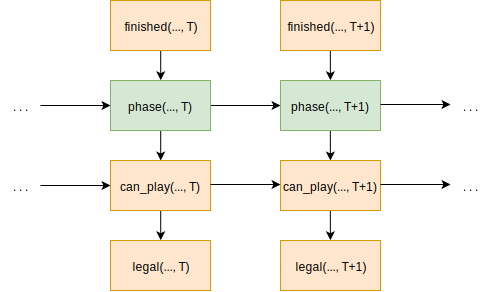
\includegraphics[width = 0.7\hsize]{figures/general_dependancies.png}
\caption{Dependency diagram between the main predicates that define \texttt{legal/3}. We need to learn the definitions of the predicates in orange.}
\label{fig:general_dependencies}
\end{figure}

\subsection{Three points of views}

Now that we know exactly which predicates we need to learn, we define three different ways of learning them in practice.

\subsubsection{Omniscient point of view}

In an \textit{omniscient point of view}, we have access to all the information regarding \texttt{legal/3}, \texttt{can\_play/3} and \texttt{finished/2}. Then, according to figure \ref{fig:general_dependencies}, we can start by learning the definition of \texttt{finished/2}. Then we can put the hypothesis found in the background knowledge in order to learn \texttt{can\_play/3}, and repeat this procedure to learn \texttt{legal/3}. 

\subsubsection{External point of view}

The \textit{external point of view} is the opposite of the omniscient point of view: we only know if a given action is legal or not. This means we do not have any information about the predicates \texttt{can\_play/3} and \texttt{finished/2}, and we have to learn all the predicates at once.

\subsubsection{Intermediate point of view}

The \textit{intermediate point of view} is a tradeoff between the two previous ones: we learn all the predicates at the same time and we have access to all the information regarding the three predicates.

\section{Implementation}

\subsection{Interface}

%TODO : reference pygame/ILASP (oracle) -> comparer méthode
We developed an basic interface in \texttt{pygame} which simulates two players  trying to play a game without knowing the rules. Each time they perform an action, an oracle tells if the action is valid or not. At each time step, an example is generated according to what the oracle says. Then this example is added to all the previous ones. Finally, we run ILASP (at each time step) for a background knowledge that describes game, for all the examples so far, and for one of the three points of views described in the previous section.

\subsection{Generating Examples}


\subsection{Reducing the hypothesis space}

%TODO difference de temps
We already know some dependencies (see figure \ref{fig:general_dependencies}). As a consequence, we can directly reduce the hypothesis space, and the number of variables per hypothesis. For example, as we know that the predicates \texttt{can\_play(Player, action, T)} and  \texttt{role(Player, Color)} will appear in the body of the rule defining \texttt{legal(Player, action(X, Y), T)}, we can write in the background knowledge:\newline
\begin{tabular}{lr}
\texttt{legal(P, action(X, Y), T) :-} & \makecell[tl]{\texttt{legal\_p(Color, action(X, Y), T),}\\ \texttt{role(P, Color), can\_play(Player, action, T).}}\\
\end{tabular}
And then we can learn this new predicate \texttt{legal\_p/3} (\texttt{p} for "partial"). 

\begin{remark}
In the two games under study, the predicates that define the states of the game only depend on the color of the pawns (and not on the players). That is why we have  \texttt{legal\_p(Color, action(X, Y), T)} in the rule above, instead of \texttt{legal\_p(Player, Color, action(X, Y), T)}.
\end{remark}

\section{Results}

\subsection{Five Field Kono}

\subsubsection{Dependencies}

The dependency diagram for Five Field Kono \texttt{legal/3} (see figure \ref{fig:FFK_dependencies}), is simpler than the one presented in figure \ref{fig:general_dependencies}. Indeed, Five Field Kono is a single-phase game, so we do not need to define a predicate \texttt{phase/2}.

\begin{figure}[h]
\centering
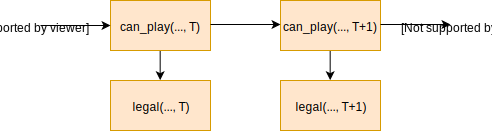
\includegraphics[width = 0.7\hsize]{figures/FFK_dependancies.png}
\caption{Dependency diagram for \texttt{legal/3} in Five Field Kono. We need to learn the definitions of both \texttt{legal/3} and \texttt{can\_play/3}.}
\label{fig:FFK_dependencies}
\end{figure}

\subsubsection{Hypothesis we are looking for}

These fact and rules describe precisely what a legal action is:\newline
\begin{tabular}{rl}
\texttt{can\_play(player1, move, 1).} & \\
\texttt{can\_play(P, move, T+1) :-} & \makecell[tl]{\texttt{can\_play(P2, move, T),}\\ \texttt{opponent\_player(P, P2), time(T).}} \\
\texttt{legal(P, move(X, Y), T) :-} & \makecell[tl]{\texttt{diagonal\_move(X, Y), holds(cell(X, S), T),} \\ \texttt{holds(cell(Y, empty), T), role(P, S),}\\ \texttt{time(T), can\_play(P, move, T).}}
\end{tabular}

The \texttt{can\_play/3} predicate is here to make \texttt{player1} start, and to prevent anyone from playing twice in a row. In addition, with this definition of \texttt{legal}, a player \texttt{P} is allowed to move a pawn from \texttt{X} to \texttt{Y} if and only if at time \texttt{T}, \texttt{Y} is empty, \texttt{P} is allowed to play, and there is a pawn in \texttt{X} that belongs to \texttt{P}.

\subsubsection{Learning the rules progressively}

%legal(player1,move(coord(1,0),coord(2,1)),1)

%legal(player2,move(coord(4,0),coord(3,1)),2)

% legal(player1,move(coord(2,1),coord(2,2)),3) tries to move a pawn to a non diagonal place.

% legal(player1,move(coord(2,1),coord(3,0)),3) tries to move green on red

\bigskip

\begin{tabular}{c|c|c|c}
step & action & meaning & hypothesis \\
\hline
\hline
1 & 0 & 0 & 
\makecell[l]{
\texttt{can\_play\_p(player1, move, 1).}\\
\texttt{legal\_p(V2, move(V0, V1), V3) :- diagonal\_move(V0, V1), }\\
\tab \texttt{holds(cell(V0,V2), V3).}
}\\
\hline
2 & 0 & 0 & 
\makecell[l]{
\texttt{can\_play\_p(player1, move, 1).}\\
\texttt{can\_play\_p(player2, move, 2).}\\
\texttt{legal\_p(V2, move(V0, V1), V3) :- diagonal\_move(V0, V1),} \\\texttt{ \tab holds(cell(V0,V2), V3).}}\\
\hline
3 & 0 & 0 & 
\makecell[l]{
\texttt{can\_play\_p(player1, move, 1).}\\
\texttt{can\_play\_p(V0, move, V2+1) :- opponent\_player(V0, V1),} \\
\tab \texttt{can\_play(V1, move, V2).}\\
\texttt{legal\_p(V2, move(V0, V1), V3) :- diagonal\_move(V0, V1), }\\
\tab \texttt{holds(cell(V0,V2), V3).}
}\\
\hline
4 & 0 & 0 & 
\makecell[l]{
\texttt{can\_play\_p(player1, move, 1).}\\
\texttt{can\_play\_p(V0, move, V3+1) :- opponent\_player(V0, V1),} \\
\tab\texttt{can\_play(V2, move, V3).}\\
\texttt{legal\_p(V2, move(V0, V1), V3) :- diagonal\_move(V0, V1),} \\
\tab \texttt{holds(cell(V0,V2), V3), holds(cell(V1,empty), V3).}
}\\
\hline
\end{tabular}

\subsubsection{Evaluation}

\subsection{Nine Men's Morris}

The rules in Nine Men's Morris are much more complicated than the rules of Five Field Kono, not only because there are more than one phase, but also because there are three different actions: placing, moving and removing a pawn.

\subsubsection{Dependencies}

This time, we need to learn all the predicates that are in figure \ref{fig:general_dependencies}. The dependency diagram for \texttt{legal/3} in Nine Men's Morris is presented in figure \ref{fig:9MM_dependencies}.

\begin{figure}[h]
\centering
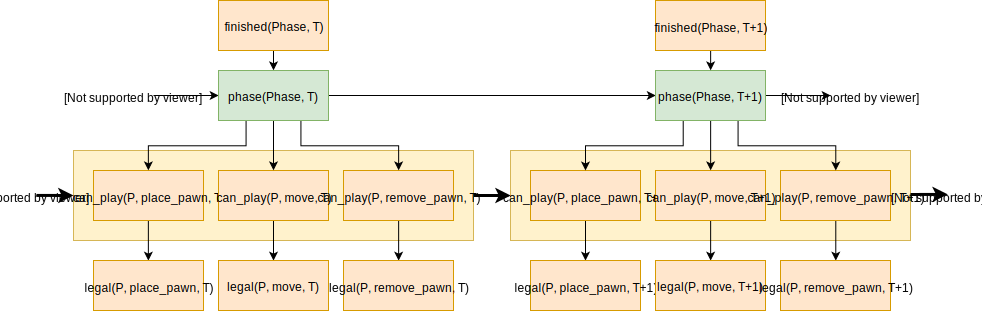
\includegraphics[width = 1\hsize]{figures/9MM_dependancies.png}
\caption{Dependency diagram for \texttt{legal/3} in Nine Men's Morris. We need to learn the definitions of \texttt{legal/3}, \texttt{can\_play/3}, and \texttt{finished/2}.}
\label{fig:9MM_dependencies}
\end{figure}

\subsubsection{Hypothesis we are looking for}

Since here we have three actions instead of only one, there are at least three rules defining \texttt{can\_play/3}, and at least three other rules defining \texttt{legal/3}.

\bigskip

Regarding the predicate \texttt{finished/2}, there is only one rule to learn:\\

\begin{tabular}{rl}
\texttt{finished(phase(1), T) :-} & \makecell[tl]{\texttt{has\_pawns(player1, 0, T), has\_pawns(player2, 0, T).}} \\
\end{tabular}

\bigskip

For the predicate \texttt{can\_play/3}, we need to learn a rule for each action (the details explaining the definitions of \texttt{can\_play/3} can be found in the previous chapter):\\

%can\_play(P1, place\_pawn, T+1) :- does(P2, Action, T), time(T), not has\_new\_mill(P2, T+1), opponent\_player(P1, P2), phase(phase(1),T+1).
%can\_play(P1, move, T+1) :- does(P2, Action, T), time(T), not has\_new\_mill(P2, T+1), opponent\_player(P1, P2), phase(phase(2),T+1).
%can\_play(P1, remove\_pawn, T+1) :- does(P1, Action, T), time(T), has\_new\_mill(P1, T+1), role(P1, C1).

\begin{tabular}{rl}
\texttt{can\_play(P1, place\_pawn, T+1) :-} & 
\makecell[tl]{
\texttt{can\_play(P2, Action, T),}\\ \texttt{opponent\_player(P1, P2),}\\ 
\texttt{not has\_new\_mill(P2, T+1),} \\
\texttt{phase(phase(1),T+1), time(T).}} \\\\

\texttt{can\_play(P1, move, T+1) :-} & 
\makecell[tl]{
\texttt{can\_play(P2, Action, T),}\\ \texttt{opponent\_player(P1, P2),}\\ \texttt{not has\_new\_mill(P2, T+1),}
\\ \texttt{phase(phase(2),T+1), time(T).}} \\\\

\texttt{can\_play(P1, remove\_pawn, T+1) :-} & 
\makecell[tl]{
\texttt{can\_play(P1, Action, T), role(P1, C1),}\\ 
\texttt{has\_new\_mill(P1, T+1), time(T).}} \\\\

\texttt{has\_new\_mill(Player, T) :-} & 
\makecell[tl]{
\texttt{has\_mill(Player, Mill, T),}\\ 
\texttt{not has\_mill(Player, Mill, T-1).}} \\
\end{tabular}

\bigskip

Finally, for \texttt{legal/3} there is also at least a rule for each action: two for removing a pawn and one for placing or moving a pawn. As usual, a player is only allowed to place or move one of his own pawns to an empty place, and the only pawns he is allowed to remove are his opponent's:

\bigskip



\begin{tabular}{rl}
\texttt{legal(P, place\_pawn(C), T) :-} & 
\makecell[tl]{
\texttt{holds(cell(C,empty),T), role(P, Color),}\\
\texttt{can\_play(P, place\_pawn, T).}
} \\\\

\texttt{legal(P, move(C1, C2), T) :-} & 
\makecell[tl]{
\texttt{holds(cell(C1, Color),T),}\\
\texttt{holds(cell(C2,empty),T), role(P, Color),}\\
\texttt{adjacent(C1,C2), can\_play(P, move, T).}}\\\\

\texttt{legal(P, remove\_pawn(C), T) :-} & 
\makecell[tl]{
\texttt{holds(cell(C,Color\_2),T), not is\_in\_mill(C, T),}\\
\texttt{opponent\_color(Color, Color\_2),}\\
\texttt{can\_play(P, remove\_pawn, T), role(P, Color).}} \\\\

\texttt{legal(P, remove\_pawn(C), T) :-} & 
\makecell[tl]{
\texttt{holds(cell(C, Color\_2),T),}\\
\texttt{opponent\_player(P1, P2), role(P2, Color\_2),}\\
\texttt{all\_in\_mill(P2, T), role(P, Color),}\\
\texttt{can\_play(P, remove\_pawn, T).}
} \\\\
\end{tabular}


\subsubsection{Learning the rules progressively}

\begin{tabular}{c|c|c|c}
step & action & meaning & hypothesis \\
\hline
\hline
1 & 0 & 0 & 0\\
\hline
\end{tabular}

\subsubsection{Evaluation}



\begin{comment}
\section{General Idea}

We observe people playing the game, and \\
if they do a valid action - positive example\\
if they do an action that is not legal - negative example\\

\bigskip

goal : learning legal/3 predicate (according to the structure of GDL)

\bigskip

source:  has been made in ILASP (paper reference)%(or concurrent) papers 

\bigskip

Learning predicate wins/2 ?

\section{Evaluation}

Evaluation at least for Five Field Kono.

\bigskip

\begin{tabular}{|c|c|c|}
\hline 
added example & hypothesis found & time (s) \\ 
\hline 
\hline
• & • & • \\ 
\hline 
• & • & • \\ 
\hline 
\end{tabular} 
\end{comment}